\chapter{Introduction to the $\Lambda$CDM Model} \label{Capitolo 1}

In this chapter we are going to introduce the basics for describing and understanding the standard cosmological model. The fundamental components of the universe according to the $\Lambda$CDM model and the equations underlying it will be introduced, like Friedmann equations (ref. \cite{Friedmann-1922}). Linear and non-linear perturbations in the cosmological standard model are also described and, finally, we will briefly discuss the need to study dark matter in more depth to resolve those tensions still present within the standard cosmological model.

\section{Introduction to cosmology}
The $\Lambda$CDM model is a well-established framework that describes the universe in cosmological terms. This model accurately explains several observations at different scales, such as Cosmic Microwave Background (CMB hereafter) (ref. \cite{Planck2020}, \cite{Nature_dark_matter_simulation}) and the large-scale structure of the universe.
In cosmology, we assume the following principles:
\begin{enumerate}
    \item \textit{Copernican Principle}\\There is no privileged system from which to observe the universe.
    \item \textit{Cosmological Principle}\\The universe can be considered isotropic and homogeneous.
\end{enumerate}
One of the most important solutions of the Einstein field equation is the Friedmann-Lema\^itre-Robertson-Walker equations (FLRW equations) that give us a metric that we can use to describe the geometry of the universe; this metric can be expressed in spherical coordinates as follows:
\begin{equation}
    ds^2 = -c^2 dt^2 + a(t)^2 \qty[\frac{dr^2}{1-kr^2} + r^2 d\theta^2 + r^2 \sin^2{\theta} d\varphi^2],
\end{equation}
which can be rewritten using the solid angle $d\Omega$ as
\begin{equation} \label{FLRW metric}
    ds^2 = -c^2 dt^2 + a(t)^2 \qty[\frac{dr^2}{1-kr^2} + r^2 d\Omega^2].
\end{equation}
Here, $t$ is the cosmological time measured by an observer at rest in the comoving system, $(r, \theta, \varphi)$ are comoving coordinates that do not change with time, and $a(t)$ is the scale factor that determines the expansion of the universe (which by convention is between 0 and 1). According to equation \eqref{FLRW metric}, the geometry of the universe is determined by the parameter $k$, which can take three possible values: $-1$, $0$, or $+1$. In other words, two objects do not change their coordinates over time, but space-time itself expands between them.\\ We can write Hubble's law
\begin{equation} \label{Hubble law}
    v = H(t) D,
\end{equation}
where $H(t)$ is the Hubble parameter, measured with the following equation
\begin{equation}
    \label{Hubble's parameter}
    H(t) = \frac{\dot{a}}{a}.
\end{equation}
It's also common and useful to indicate the Hubble parameter at the present time with $H_0$ with a value constrained by CMB observations to $H_0 = (67.66 \pm 0.42) \ \text{km} \; \text{s}^{-1} \; \text{Mpc}^{-1}$ (ref. \cite{Planck2020}).\\
This Hubble parameter helps us to obtain an estimate of the age of the universe, thanks to the following simple formula
\begin{equation}
    \label{Hubble time}
    t_0 = \frac{1}{H_0} \simeq 14 \; \text{Gyr},
\end{equation}
also known as "Hubble time". This is a very good value, close to the data estimating the age of the universe at $13.8 \hspace{0.5mm} \; \text{Gyr}$.\\ Now, if we consider a space-time point with coordinates $(r, \theta, \varphi) = (0,0,0)$, which corresponds to our position, and a second space-time point at $(r, \theta, \varphi) = (r_\star, 0, 0)$, we can calculate the distance between them as follows:
\begin{equation}
    l = \int_{0} ^{r_\star} dl.
\end{equation}
Using the FLRW metric, we obtain
\begin{equation}
    l = \int_{0} ^{r_\star} dl = a(t) \int_{0} ^{r_\star} \frac{dr}{\sqrt{1-kr^2}} = a(t) \int_{0} ^{r_\star} dr = a(t)r_ \star,
\end{equation}
now, differentiating both sides with respect to time, we get
\begin{equation}
    \frac{dl}{dt} = \dot{l}=\dot{a} \int_{0} ^{r_\star} \frac{dr}{\sqrt{1-kr^2}} = \dot{a} \frac{l}{a},
\end{equation}
where for $k=0$ (ref. \cite{de_Bernardis_2000}), the equation simplifies to
\begin{equation}
    \dot{l} = \frac{\dot{a}}{a}l \quad \Longrightarrow \quad v = H(t) D.
\end{equation}
In an expanding Universe, light emitted by distant sources undergoes a phenomenon known as redshift. This effect is conceptually similar to the Doppler effect experienced by sound waves, where the frequency changes due to the relative motion between the source and the observer. However, in the cosmological context, redshift is primarily caused by the expansion of spacetime itself, as described by the scale factor \( a(t) \) in the metric.

Let us consider a light ray emitted at time \( t_e \) by a distant source with wavelength \( \lambda_e \), and received at a later time \( t_o \) by an observer, who measures a wavelength \( \lambda_o \). Due to the expansion of the universe during the light's travel, the observed wavelength \( \lambda_o \) will be stretched compared to the emitted one. This leads to the definition of the redshift \( z \) as:
\begin{equation} \label{redshift definition}
1 + z = \frac{\lambda_o}{\lambda_e} = \frac{a(t_o)}{a(t_e)},
\end{equation}
where \( a(t_e) \) and \( a(t_o) \) are the values of the scale factor at the time of emission and observation, respectively. Thus, the redshift provides a direct measure of how much the Universe has expanded during the propagation of the light.\\

\section{Friedmann equations}
In general relativity, the relation between the space-time and  matter/energy is given by Einstein's field equation
\begin{equation}
    R_{\mu \nu} - \frac{1}{2}g_{\mu \nu}R + g_{\mu \nu}\Lambda = \frac{8 \pi G}{c^4} T_{\mu \nu},
\end{equation}
where $R_{\mu \nu}$ is the Ricci tensor, $g_{\mu \nu}$ is the metric tensor and $T_{\mu \nu}$ is the stress-energy-momentum tensor.
The energy can be described as a perfect fluid characterized by an energy-momentum tensor
\begin{equation}
    T_{\mu \nu} = p g_{\mu \nu} + c^2 \qty(\frac{p}{c^2} + \rho) u_{\mu} u_{\nu},
\end{equation}
where $p$ is the pressure, $\rho$ is the density of the fluid and $u^\mu$ is the 4-velocity of the fluid.

To obtain a first approximation, we can simplify the problem and assume that all of the components of the universe are decoupled and they evolve independently. 
The conservation equation is given by the application of the covariant derivative with the FLRW metric $\nabla _\mu T^{\mu \nu} = 0$ with $\nabla _\mu$ covariant derivative.
The result is:
\begin{equation} \label{equation of state}
    \dot{\rho} + 3 \frac{\dot{a}}{a} \qty(\rho + \frac{p}{c^2}) = 0,
\end{equation}
if we assume $p = \rho w$ with $w$ a constant equation of state. Substituting in \eqref{equation of state} and integrating it is possible to find $\rho(a)$
\begin{equation}\label{integrated equation of state}
    \rho(a) \propto a^{-3(1+w)},
\end{equation}
so the three scenarios are the following:
\begin{itemize}
    \item Radiation: $w = \frac{1}{3}$
    \item Matter: $w = 0$
    \item Cosmological constant ($\Lambda$): $w = -1$
\end{itemize}

From the FLRW metric and General Relativity, we derive two fundamental equations, known as the Friedmann equations (ref. \cite{Friedmann-1922}):
\begin{equation} \label{Friedmann equations with dark energy}
    \left\{
    \begin{aligned}
        \left( \frac{\dot{a}}{a} \right)^2 &= \frac{8\pi G}{3} \rho - \frac{k c^2}{a^2} + \frac{\Lambda c^2}{3}, \\  
        \frac{\Ddot{a}}{a} &= - \frac{4\pi G}{3c^2}(\rho c^2 + 3p) + \frac{\Lambda c^2}{3}.
    \end{aligned}
    \right.
\end{equation}
These equations determine the evolution of the scale factor as a function of radiation and matter content in the universe. The density is the sum of radiation density, matter density (baryonic and dark matter) and the last term is the dark energy.
In \eqref{Friedmann equations with dark energy} $\dot{a}$ represents the time derivative of $a$, while $\rho$ accounts for both matter and radiation density, and $p$ is the pressure. This set of equations describe the evolution of the universe in terms of the scale factor $a(t)$ and the parameter $k$. It is also very important to note the negative sign in the second equation, as this is the reason why the velocity of expansion can rapidly slow down in a universe without dark matter. Another crucial aspect is the squared term in the first Friedmann equation, which allows the derivative of the scale factor to be either positive or negative. In other words, the universe can be either expanding or contracting (Friedmann's equations do not prohibit this possibility).\\
We can also identify the cosmological constant as an energy density
\begin{equation}\label{dark energy}
    \rho_\Lambda = \frac{c^2}{8 \pi G} \Lambda,
\end{equation}  
and it's very important to notice that the dark energy density remains constant.\\

Thanks to Hubble's studies and numerous observations, we now know that the universe is expanding.
Within these equations, we can introduce another important parameter using equation \eqref{Hubble's parameter}
\begin{equation} \label{critical density}
    \rho_{crit} = \frac{3H^2(t)}{8 \pi G},
\end{equation}
this is the critical density (also called $\rho_c$ in this thesis), which allows us to define the density parameter $\Omega$ as follows
\begin{equation}
    \label{Omega definition}
    \Omega = \frac{\rho}{\rho_{crit}}.
\end{equation}
which is particularly useful as it establishes a direct relationship between the density of the universe and its geometry. As previously discussed, there are three possible cases:
\begin{itemize}
    \item If $k = -1$, then $\Omega < 1$ and $\rho < \rho_{crit}$.\\
    In this case, the universe has negative curvature and follows a hyperbolic geometry (similar to a saddle shape).
    \item If $k = 0$, then $\Omega = 1$ and $\rho = \rho_{crit}$.\\
    In this scenario, the universe is flat.
    \item If $k = +1$, then $\Omega > 1$ and $\rho > \rho_{crit}$.\\
    Here, the universe has positive curvature and is closed with a spherical geometry.
\end{itemize}
As before, we want to rewrite the Friedmann equation introducing $\Omega$.\\ The Friedmann equation \eqref{Friedmann equations with dark energy} became 
\begin{equation}
    \frac{H^2}{{H_0}^2} = \frac{\rho_m}{\rho_{crit, 0}} + \frac{\rho_r}{\rho_{crit, 0}} + \frac{\Lambda}{\rho_{crit,0}} = \Omega_m + \Omega_r + \Omega_\Lambda,
\end{equation}
the left side term is equal to one because it's calculated at present time and $\rho_{crit, 0}$ is the critical density calculated at present time.\\
With this notation the relation between the three parameters is obviously given by $\Omega(t) = \Omega_m (t) + \Omega_r (t) + \Omega_\Lambda (t)$ and $\Omega_k$ associated at the curvature is $\Omega_k (t) = - \frac{k}{H(t)^2 a^2} = 1 - \Omega (t)$. Thanks to these relations we can rewrite the first Friedmann equation:
\begin{equation}
    H^2 (t) = H_0^2 [\Omega_m (1+z)^3 + \Omega_r (1+z)^4 + \Omega_\Lambda +(1-\Omega)(1+z)^2].
\end{equation}

\begin{figure}[h!]
\centering
    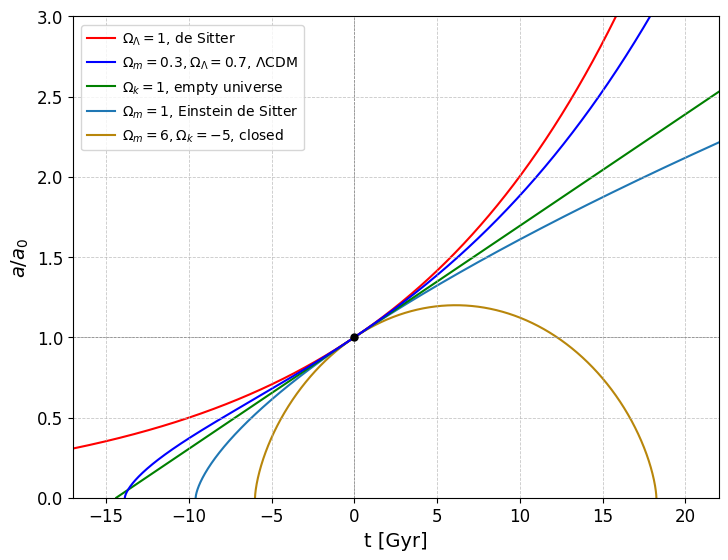
\includegraphics[width=0.6\linewidth]{Images/Chapter1/evolution of universe.png}
    \caption[Evolution of universe in different regime]{Evolution of the scale factor as a function of time in different type of universe. Credits \cite{geek3_universe_scale}.}
\label{different universe - scale factor}
\end{figure}

It has been said before that the solution of the covariant derivative of the stress-energy tensor depends on a parameter $w$. 
An analytical solution for the scale factor can be derived by assuming that only one of the components with equation of state dominates the energy density.

In the early universe, after the Big Bang, the radiation contribution is more important than the contribution of matter and this is also called the radiation dominated era. In this epoch the density falling down very quickly: $\rho(a) \propto a^{-4}$. The radiation density has decreased enough to allow it to take over to matter, ushering in the matter dominated era where the density scale with the following trend: $\rho (a) \propto a^{-3}$.\\ So, immediately after the explosion, the universe entered a radiation-dominated era, during which it expanded slowly ($\propto t^{\frac{1}{2}}$) while the density decreased rapidly. As the universe expanded, the gas cooled, leading to the matter-dominated era. In this era, according to the Friedmann equations, the expansion occurred at a faster rate ($\propto t^{3/2}$), while the matter density decreased more slowly.\\ Recently we entered in the dark energy (DE) era where the DE is responsible for the expansion of the universe as we can easily see in fig. \ref{Evolution of cosmic components} in the lower right part.

\begin{figure}[h!]
\centering
    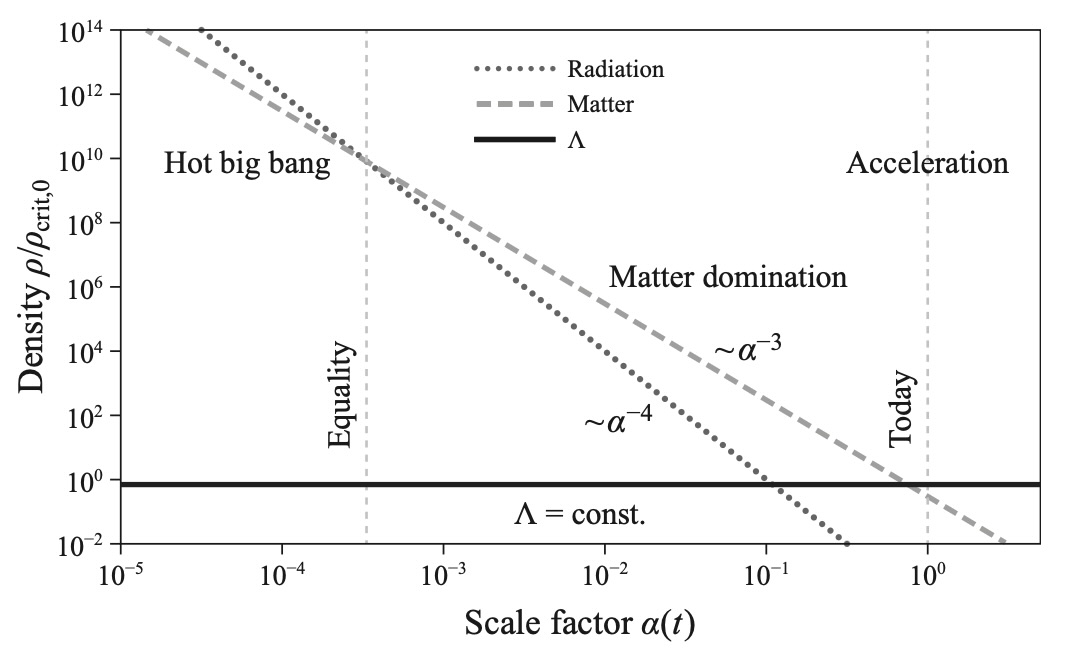
\includegraphics[width=0.62\linewidth]{Images/Chapter1/Evolution of elements in universe.jpeg}
    \caption[Evolution of cosmic components]{Evolution of cosmic components (radiation, matter and dark energy). The vertical lines mark the different eras. Fig. 5.2 in ref. \cite{2024darkmatter}.}
\label{Evolution of cosmic components}
\end{figure}

\section{Perturbations and their evolution}

\subsection{Linear perturbation}
After the Big Bang, the universe underwent an early phase dominated by radiation, during which density fluctuations could not grow significantly due to the strong radiation pressure. As the universe expanded and cooled, it transitioned to a matter-dominated phase, allowing these primordial fluctuations to start growing under gravity.\\
Around redshift $z \sim 1100$ (ref. \cite{2024darkmatter}), during the epoch of recombination, the universe became transparent to radiation: photons decoupled from matter and the cosmic microwave background (CMB) was released. The CMB provides a snapshot of the universe at that time, and its tiny temperature anisotropies (of the order of $\mu$K, see fig. \ref{Planck CMB}) reflect the initial density perturbations in the primordial plasma.\\
In fact, if the cosmological principle were perfectly respected and the distribution of matter and energy in the universe were really isotropic and uniform, the cosmic structures we currently observe would not exist.

\begin{figure}[h!]
\centering
    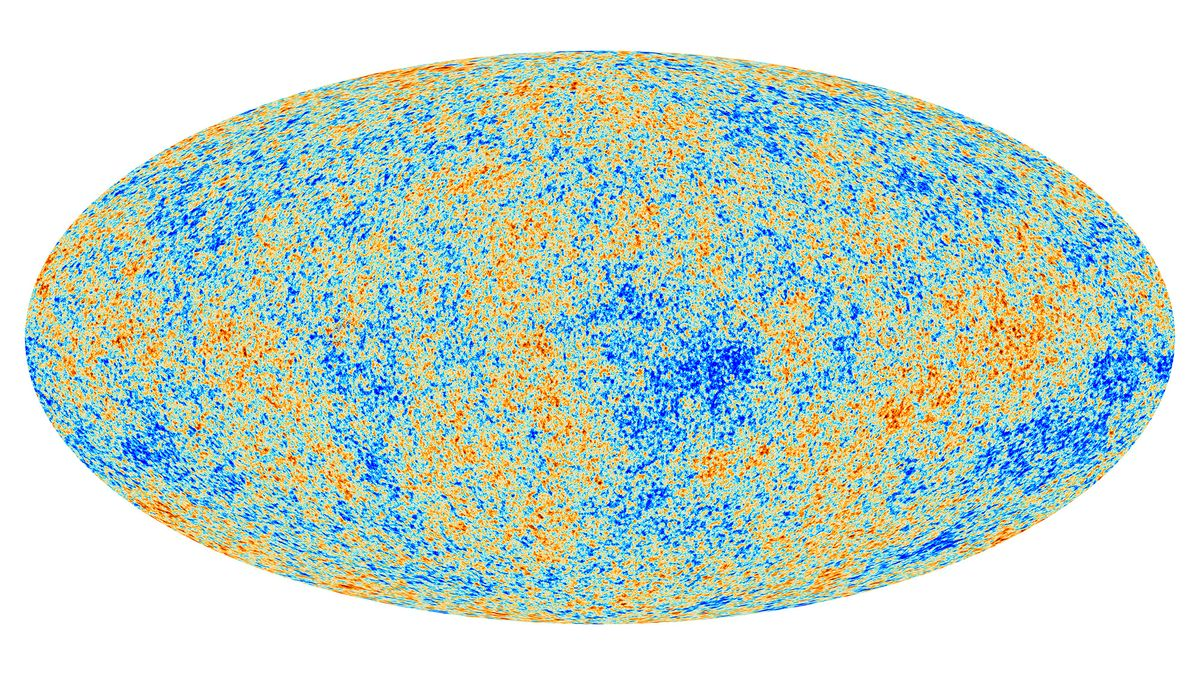
\includegraphics[width=0.60\linewidth]{Images/Chapter1/Planck CMB.jpg}
    \caption[CMB image obtained by the Planck satellite]{Temperature anisotropies in the cosmic microwave background.\\ This image is based on data from the Planck release, published in 2013. Credits \cite{planckSatelliteImage}.}
\label{Planck CMB}

\end{figure}
In a universe governed by non-relativistic matter, perturbations grow over time. Areas with a higher density of matter attract other matter, while regions with lower densities "empty" themselves. This is called gravitational instability and it is a crucial concept for understanding the processes that explain the formation of cosmic structures. However, the expansion of the universe damps the growth of these perturbations, preventing exponential growth and reducing the efficiency of gravitational collapse.
The structure we observe today is assumed to have grown from small initial density perturbations in the density field due to the action of gravity. If the perturbations (shown in fig. \ref{Planck CMB}) are very small, about $\frac{\delta T}{T} \sim \frac{\delta \rho}{\rho} \sim 10^{-5}$, as mentioned earlier, we can consider the contents of the universe as a perfect fluid characterized by pressure $p(\vec{x}, t)$ and density $\rho (\vec{x}, t)$. Assuming a non-relativistic fluid, the evolution of the fluid is described by the continuity equation
\begin{equation}
    \frac{D \rho}{dt} + \rho \nabla \cdot {\Vec{u}} = 0.\footnote{Where $\frac{D}{dt}$ indicate the convective derivative define as $\frac{D}{dt} = \frac{\partial}{\partial t} + \vec{v} \cdot \nabla$.}
\end{equation}
The perturbation of $\rho(\vec{x}, t)$ can be written as $\delta\rho(\vec{x}, t) = \rho (\vec{x}, t) - \Bar{\rho} (t)$ (deviation from mean density) where $\Bar{\rho}(t)$ is the density background.\\ We can still write the density $\rho (\vec{x}, t)$ in this epoch of the universe as $\rho (\Vec{x},t) = \Bar{\rho}(t) (1 - \delta(\Vec{x},t))$.\\
Other necessary equation is the Euler's equation
\begin{equation}
    \frac{D \Vec{u}}{dt} = - \frac{1}{\rho} \nabla p - \nabla \Phi,
\end{equation}
where $\Phi$ is the gravitational potential associated with the Poisson equation
\begin{equation} \label{Poisson equation}
    \nabla^2\Phi = 4 \pi G \rho.
\end{equation}
One last equation is needed to close the system: the equation of state, which links pressure to density.\\ In particular, if the evolution of perturbation is adiabatic, $p(\rho, S)$ is equal to zero for dark matter and $p(\rho, S) \neq 0$ for baryonic matter and/or radiation.

The evolution of linear perturbations is governed by the combination of the previous equation that results in the following:
\begin{equation}
    \Ddot{\delta_k} + 2H \dot{\delta_k} + \delta_k \qty[\frac{k^2 {v_s}^2}{a^2} - 4 \pi G \Bar{\rho}] = 0,
\end{equation}
where $v_s$ is the sound speed in the fluid and $a$ is the scale factor. This equation describes the evolution of perturbations in the early universe in the linear regime.
We now move to Fourier space to solve the differential equations:
\begin{equation}
    \delta_{\vec{k}} (t) = \qty(\frac{1}{2 \pi})^3 \int \delta(\vec{y}, t) e^{-i \vec{k} \cdot \vec{y}} d^3 y,
\end{equation}
where $\vec{k} = \frac{2 \pi}{\lambda}$.\\
A particular scale exists, called the Jeans scale, which corresponds to the point where the term in brackets vanishes
\begin{equation}
    K_J = a\sqrt{\frac{4 \pi G \Bar{\rho}}{{v_s}^2}}.
\end{equation}
This marks a transition regime. For scales smaller than the Jeans scale (i.e., $k > K_J$), pressure dominates; for $k < K_J$, gravity dominates and perturbations begin to grow.
Initially, the Jeans scale is very large, and all small perturbations cannot grow because pressure would erase them. After the reionization era\footnote{In cosmology, the era of reionization is the period following the big bang during which the mass of hydrogen that filled the universe became transparent to electromagnetic radiation.}, the Jeans scale drops quickly and perturbations can grow. Another important aspect that we have to consider is the free-streaming damping: particles with high velocity can move from regions with high density to regions with small density and vice-versa. This effect calms the disturbances.
If there are particles moving freely in the universe, it doesn't mean they will necessarily come together under the force of gravity. This is a scale called free-streaming scale, which is the distance that a dark matter particle can travel in a certain amount of time. Below this scale, even dark matter perturbations cannot grow because the particles move in a way that prevents them from clustering. This minimum scale depends on the mass of dark matter particles.\\ According to observation, we can see that small structures formed first, with dark matter halo having a mass of about $10^6 M_\odot$. This is very important because it tells us that particles with a very small mass, like neutrinos, cannot make up dark matter. They would produce much larger structures and would have a much higher free-streaming scale. This suggests that dark matter particles must be very massive and move slowly; this is what we call cold dark matter.\\ These structures grow in a hierarchical way. Baryons particles fall into the gravitational potential of dark matter if the structures are dense enough. As they fall, the density and pressure increase, which also raises the temperature. In this condition, the first stars begin to form.
As we have seen before, radiation density decreases very quickly ($\rho \propto a^{-4}$) while matter density decreases much more slowly ($\rho \propto a^{-3}$).
At a certain point, we reach the so-called matter-radiation equality, when the density of matter equals the density of radiation
\begin{equation}
    \Omega_m (1+z)^3 = \Omega_r (1+z)^4,
\end{equation}
where $z$ is called the redshift of equality, with a value of approximately $z \sim 3400$ (see fig. \ref{Evolution of cosmic components}) according to ref \cite{2024darkmatter}. From this moment, the universe entered the matter dominated era.
In the linear regime, the solution for the perturbation in Fourier space can be rewritten as:
\begin{equation}
    \delta_{\vec{k}} (t) = \delta_{\vec{k}_{\text{in}}} \, D(t),
\end{equation}
where the first term depends only on $\vec{k}$ (these are the initial perturbations observed in the cosmic microwave background), and the second term is called the linear growth factor ($D(t)$).
The latter has two possible solutions \footnote{Assuming a universe with $k=0$ and matter dominated.}:
\begin{equation}
\begin{split}
    D_{-} (t) &\propto H(t) \propto t^{-1},\\
    D_{+} (t) &\propto H(t) \int_{0} ^{t} \frac{dt'}{a^2(t') H^2(t')} \propto t^{\frac{2}{3}}.
\end{split}
\end{equation}
Therefore, perturbations do not grow linearly in time; their growth is somewhat slower.
It is important to note that even if the universe were not expanding, and even if dark matter had no pressure, not all structures could form. Only structures above a certain mass scale can form because the free streaming of the dark matter still resists gravitational collapse.\\


\subsection{Relativistic perturbation}

The relativistic theory of cosmological perturbations provides the most general and rigorous framework for studying the evolution of inhomogeneities in the Universe. Derived directly from general relativity, it overcomes the limitations of the Newtonian approximation and is valid across all scales and cosmic epochs. This formalism allows for a consistent treatment of scalar, vector, and tensor perturbations.
In particular, the scalar perturbations, which are the most relevant for structure formation, are often analyzed in the conformal Newtonian gauge. This gauge simplifies the metric perturbation expressions by introducing two scalar potentials, $\phi$ and $\psi$, directly related to the Newtonian gravitational potential and spatial curvature perturbation. 

It's possible to construct this formalism by introducing a perturbed metric tensor:
\begin{equation}
    g_{\mu \nu} = \Bar{g}_{\mu \nu} + \delta g_{\mu \nu},
\end{equation}
where $\delta g_{\mu \nu}$ is the perturbation that can be written as the sum of several contributions: $\delta g_{\mu \nu}^S$, $\delta g_{\mu \nu} ^V$, and $\delta g_{\mu \nu} ^T$ thanks to the decomposition theorem\footnote{In the first-order perturbation theory the scalar, vector and tensor part do not couple to each other according to ref. \cite{Relativistic_perturbation}.}. Here, the superscripts indicate respectively the scalar, the vector, and the tensor perturbation.\\ In order to simplify the problem, we can consider only the first scalar perturbation that can be written in terms of two potentials: $\phi$ and $\psi$.
In a suitable gauge, called a conformal Newton gauge, it is possible to define two gauge-invariant potentials, also called Bardeen potentials, with the following identities:
\begin{equation}
    \begin{cases}
    \Phi = \phi, \\
    \Psi = \psi .
    \end{cases}
\end{equation}
This leads to a particularly simple writing for the perturbative matrix we are studying
\begin{equation}
    \delta g_{\mu \nu} = \begin{pmatrix}
    -2\frac{\Phi}{c^2} & 0 \\
    0 & -2\frac{\Psi}{c^2} \delta_{ij}
\end{pmatrix}.
\end{equation}\\
Now the distance can be written in the following way
\begin{equation}
    ds^2 = g_{\mu \nu} dx^\mu dx^\nu = a^2(t) \qty[-\qty(1+2\frac{\Phi}{c^2}) c^2 dt^2 + \qty(1-2\frac{\Psi}{c^2})\delta_{ij}dx^idx^j],
\end{equation}
and rewritten in comoving spherical coordinates
\begin{equation}\label{metric with badern potential}
    ds^2 = a^2(t) \qty[-\qty(1+\frac{2\Phi}{c^2})c^2 dt^2 + \qty(1-\frac{2\Psi}{c^2}) \qty(d\chi^2+f_k^2(\chi)d\Omega^2) ],
\end{equation}
where $f_k (\chi)$ can assume three different forms
\begin{equation}
f_k(\chi) =
\begin{cases}
\sin(\chi) & \text{if } k > 0 \text{ (closed universe)} \\
\chi & \text{if } k = 0 \text{ (flat universe)} \\
\sinh(\chi) & \text{if } k < 0 \text{ (open universe)}
\end{cases}
\end{equation}

This perturbed metric is commonly used to describe astrophysical structures such as galaxy clusters. Although these systems are strongly non-linear in terms of matter overdensities (with density contrasts $\delta \gg 1$), the gravitational potential $\Phi$ remains small compared to $c^2$ (typically $\Phi/c^2 \sim 10^{-5}$), which justifies the use of linear perturbation theory for the metric.
The matter density perturbations are connected to the potentials through the Poisson equation \eqref{Poisson equation}, which comes from the "00" component of the perturbed Einstein equations.
Within the standard $\Lambda$CDM framework and assuming General Relativity with a perfect fluid, the two Bardeen potentials coincide: $\Phi = \Psi$. However, in more general theories of gravity or models with anisotropic stress, this equality can be violated. Therefore, detecting $\Phi \ne \Psi$ may provide evidence for physics beyond the $\Lambda$CDM model, such as modified gravity or exotic interactions within the dark sector.

\subsection{Non linear perturbation}

Linear perturbation theory is a good approximation only when $\delta \rho \ll 1$.
Unfortunately, actual observations suggest that structures have formed under non-linear conditions.
This forces us to investigate non-linear evolution further, which requires more complex tools.
On small scales it's possible to observe the nonlinear collapse of overdensity; this requires more complex tools to be described. This can be thought of as an overdense region that expands with the universe until it decelerates, reverses its motion, gravitationally collapses, and finally reaches virial equilibrium.
However, to understand the formation of clusters on small scales, the main approach is numerical simulation. 
These simulations can be complicated as desired by adding dark energy, baryonic matter (e.g. gas), black holes, and supernovae. However, a simpler method is to consider only dark matter. This is still a very good approximation since it allows us to study dark matter halos in which galaxies form.
The most used technique to study these problems is the simulation N-body. One of the famous N-body simulations is the millennium simulation that traced over 10 billion particles in a cube with sides approximately 2 billion light years long.
\begin{figure}[h!]
    \centering
    \includegraphics[width=1\textwidth]{Images/Chapter1/Millenium run.png}

    \vspace{2mm} % Spazio verticale tra immagine e didascalie
    \begin{minipage}[t]{0.24\textwidth}
        \centering
        $z = 18.3$\\ $(t = 0.21\text{ Gyr})$
    \end{minipage}
    \begin{minipage}[t]{0.24\textwidth}
        \centering
        $z = 5.7$\\ $(t = 1 \text{ Gyr})$
    \end{minipage}
    \begin{minipage}[t]{0.24\textwidth}
        \centering
        $z = 1.4$\\ $(t = 4.7\text{ Gyr})$
    \end{minipage}
    \begin{minipage}[t]{0.24\textwidth}
        \centering
        $z = 0$\\ $(t = 13.8\text{ Gyr})$
    \end{minipage}

    \caption[Millenium simulation of cosmic structure]{
        Evolution of the universe’s large-scale structure as simulated in the Millennium Simulation Project, shown at different redshifts ($z$). Each panel displays the distribution of dark matter on cosmological scales at a different redshift/time. Credits \cite{millennium_simulation}.}
    \label{fig:scala_cosmica_unificata}
\end{figure}

Of course, this is not the only way; another approximation used is the Zel’dovich approximation or the spherical collapse model or even the Lagrange perturbation theory. However, these, as mentioned above, are complex models that will not be addressed in this thesis.

\begin{figure}[h!]
\centering
    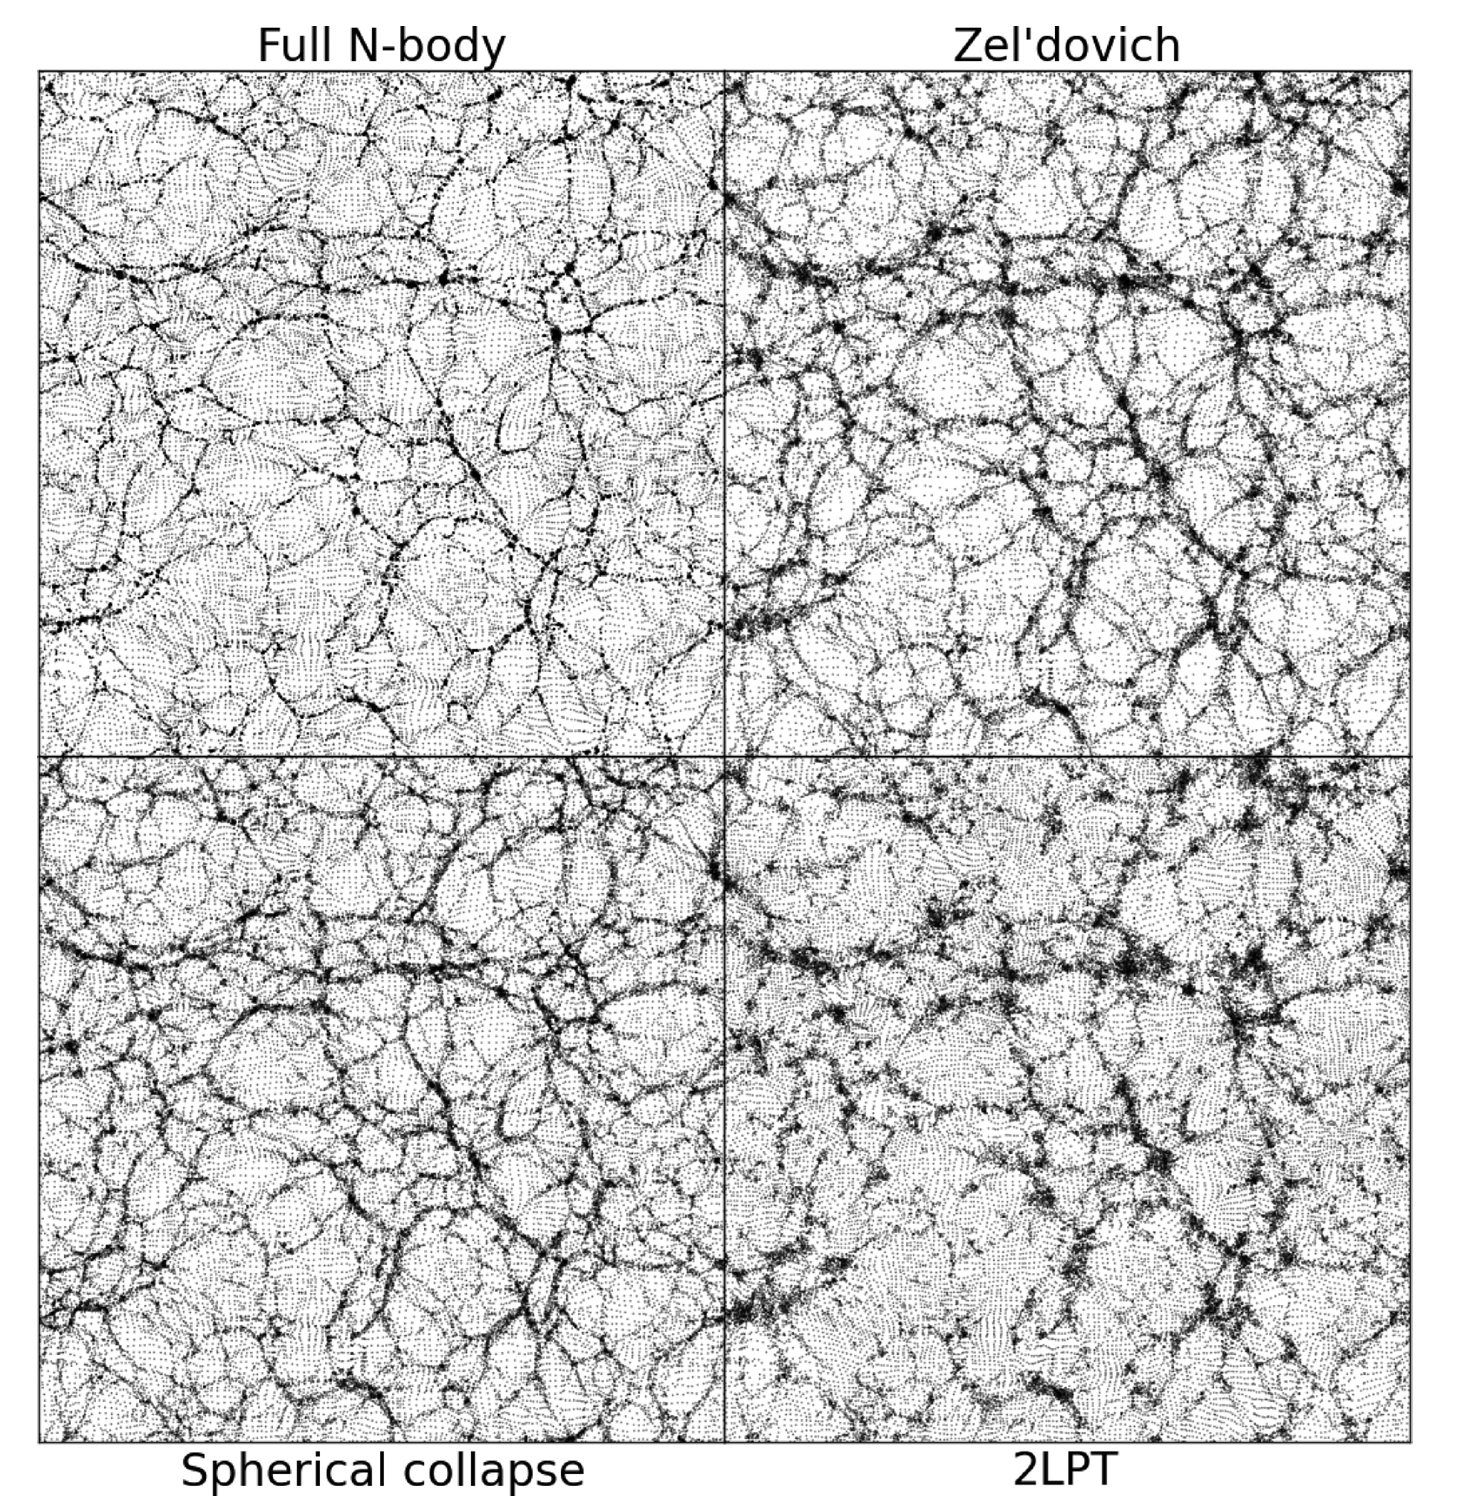
\includegraphics[width=0.55\linewidth]{Images/Chapter1/Non linear simulation.png}
    \caption[Simulations in different regime]{Top left is an N-body simulation, top right is in Zel’dovich approximation, bottom left is a simulation in spherical collapse approximation and the last bottom right frame is in lagrangian perturbation theory. Figure 10 in ref. \cite{Neyrinck-2012}.}
\label{Non linear perturbation simulaion}
\end{figure}


\section{Summary of $\Lambda$CDM model}

The $\Lambda$CDM model (Lambda Cold Dark Matter) is the current standard model of cosmology, providing a remarkably successful description of the Universe's evolution and composition. It assumes a flat universe (ref. \cite{de_Bernardis_2000}) composed of ordinary (baryonic) matter, cold dark matter (CDM), and a cosmological constant $\Lambda$ accounting for dark energy.\\
According to recent observations, the $\Lambda$CDM model describes a universe composed of approximately 31\% matter and 69\% dark energy. More precisely, the density parameters are measured to be $\Omega_m = 0.3111 \pm 0.0056$ and $\Omega_\Lambda = 0.6889 \pm 0.0056$, where $\Omega_m$ includes both baryonic and dark matter (DM) components (ref. \cite{Planck2020}). These values are derived from observations of the Cosmic Microwave Background (CMB), particularly from the Planck 2020 results (ref. \cite{Planck2020}).
While the addition of the cosmological constant is strictly necessary to explain the expansion of the universe (ref. \cite{Riess_1998_accelerating_universe}), the requirement for cold dark matter ensures the formation of large structures on cosmological scales that other types of dark matter couldn't explain.
Indeed, other types of dark matter, which will be discussed in more detail in Chapter \ref{Dark matter properties}, fail to correctly explain the formation of large-scale cosmic structures.
Dark matter is supported by a wide range of observational evidences across different scales. On galactic scales, the flat rotation curves of spiral galaxies suggest the presence of extended dark matter halos (ref. \cite{Vera-Rubin}). On the scale of galaxy clusters, gravitational lensing and velocity dispersion measurements indicate a significant amount of unseen mass (ref. \cite{Empirical_proof_DM_lensing}). Finally, on cosmological scales, dark matter is essential to explain the pattern of the CMB anisotropies and the growth of large-scale structures (ref. \cite{Planck2020}, \cite{Nature_dark_matter_simulation}).
Another crucial parameter in the $\Lambda$CDM framework is the Hubble constant $H_0$, which quantifies the current rate of expansion of the universe. The value inferred from CMB data is $H_0 = (67.66 \pm 0.42) \; \text{km} \; \text{s}^{-1} \; \text{Mpc}^{-1}$ (ref. \cite{Planck2020}). However, this measurement is in tension with values obtained through local observations, such as the study of Type Ia supernovae; in fact, recent analyses report a significantly higher value: $H_0 = 75.7^{+8.1}_{-5.5} \; \text{km} \; \text{s}^{-1} \; \text{Mpc}^{-1}$ (ref. \cite{Pascale2024SN-H0-pe-measurement-H0}).
This discrepancy, known as the Hubble tension, represents one of the most intriguing open problems in modern cosmology (see fig. \ref{Hubble tension} below).\\ Another important and recent study also observed discrepancies in dark energy, proposing that it is not truly constant (ref. \cite{DESI_DarkEnergy}). 
All these tensions suggest that our current understanding of the universe — as described by the standard $\Lambda$CDM model — might be incomplete and motivates further investigation into the nature of dark matter, dark energy and possibly new physics beyond the standard model of cosmology. In fact, the $\Lambda $CDM model still fails to provide a natural explanation for the existence and physical origin of the cosmological constant.

\begin{figure}[h!]
\centering
    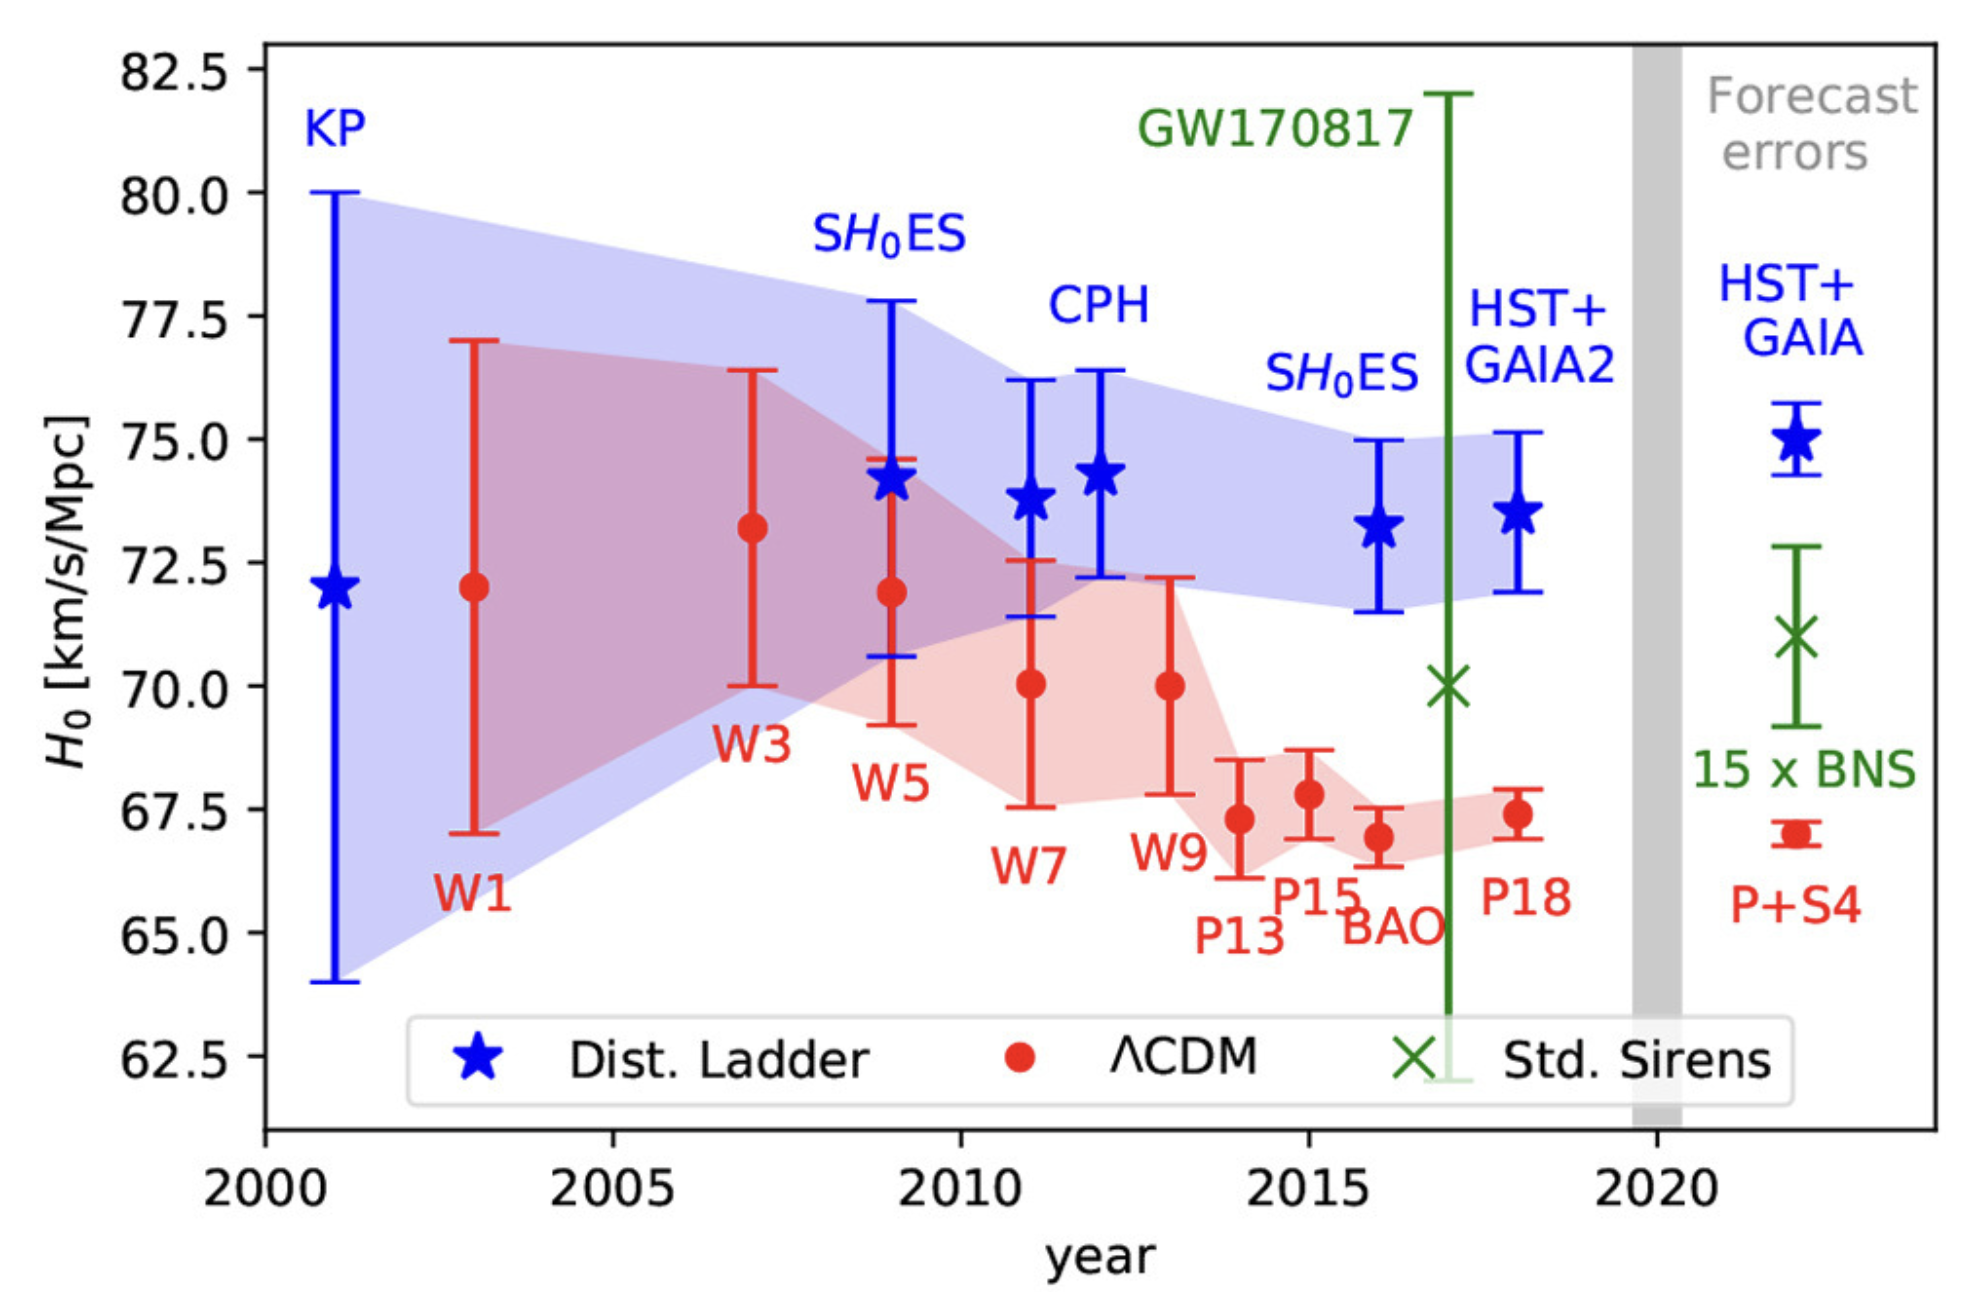
\includegraphics[width=0.60\linewidth]{Images/Chapter1/Hubble tension.png}
    \caption[Hubble tension]{The data in blue represents the measurements made with the Cepheids, those in red refer to the data obtained with the CMB and finally the green lines are the results of gravitational wave observations. Figure 8 in ref. \cite{Dark-Energy-in-Light-of-Multi-Messenger-Gravitational-Wave-Astronomy}.}
\label{Hubble tension}
\end{figure}

In particular, dark matter, which makes up the majority of the matter component in the universe, remains one of the least understood elements in the $\Lambda$CDM model. Although it works well on large scales and explains many observations, the model has several problems on smaller scales. These include the cusp-core problem, where the predicted steep density profiles in galaxy centers are not observed, and the missing satellite problem, where the simulations predict a larger number of small satellite galaxies are being detected (see Chapter \ref{Dark matter properties}).\\ These and other small-scale problems suggest that dark matter might not be entirely cold and collisionless as assumed in the standard cosmological model, but could instead possess self-interactions or exhibit different clustering behavior. Studying these tensions could thus provide crucial insights into the fundamental nature of dark matter.\\ For these reasons, in the following chapters, I will focus on the properties and distribution of dark matter, presenting more recent modeling approaches.